\subsection{Weryfikacja modelowa z zastosowaniem logiki temporalnej}

\subsubsection{Klasyczna logika zdań}

\begin{itemize}
	\item nadaje logiczny stan (prawda / fałsz) dla każdego zdania,
	\item relacje logiczne: koniunkcja, negacja, alternatywa, implikacja, równoważność.
	\item pozwala wnioskować o prawdziwości zdania.
\end{itemize}

\subsubsection{Czas}

\begin{itemize}
	\item Nieprzestrzenne kontinuum, w którym zdarzenia zachodzą w nieodwracalnej kolejności od przeszłości, przez teraźniejszość do przyszłości,
	\item Sposoby podziału czasu:
	\begin{itemize}
		\item Skończony (lewostronnie, prawostronnie lub obustronnie) i nieskończony
		\item Punktowy i przedziałowy (struktura czasowa składa się wyłącznie z punktów lub wyłącznie z przedziałów)

		\item Liniowy, rozgałęziony i równoległy.
	\end{itemize}
\end{itemize}

\subsubsection{Logika temporalna = klasyczna logika zdań + czas}

Logika temporalna jest to rozszerzenie logiki tradycyjnej o symbole określające upływ czasu. Weryfikacja modelowa pozwala odpowiedzieć na pytanie czy formalny model funkcji systemu dany jako automat spełnia własności, zdefiniowane za pomocą formuł logiki temporalnej. Główne zastosowania to:

\begin{itemize}
	\item zarządzanie temporalnymi bazami danych,
	\item opis systemów współbieżnych,
	\item opis systemów reagujących na bodźce,
	\item określanie własności systemów,
	\item automatyczna weryfikacja programów – matematyczne udowodnienie ich poprawności. \\
\end{itemize}

Najważniejsze zadania weryfikacji:

\begin{itemize}
	\item osiągalność (pożądany stan zostanie \textbf{w końcu} osiągnięty)
	\item bezpieczeństwo (gwarancja, iż stan nieprawidłowy \textbf{nigdy} nie zostanie osiągnięty)
\end{itemize}

\subsubsection{Typy logiki temporalnej}

Wyróżniamy bardzo wiele typów logiki temporalnej, m.in.:

\begin{itemize}
	\item \textbf{LTL} (\textit{Linear Temporal Logic}) – z liniową strukturą czasu,
	\item \textbf{CTL} (\textit{Computation Tree Logic}) – rozszerzenie logiki LTL o rozgałęzione warianty upływu czasu). Czas jest dyskretny, może się rozgałęziać (ale od pewnego momentu, wcześniej jest liniowy) oraz lewostronnie skończony (w przyszłości nieskończony). Zastosowanie : w działających współbieżnie programach , w systemach gdzie istnieje wiele wariantów upływu czasu,
	\item \textbf{Real Time CTL} - dalsze rozwiniecie logiki temporalnej, pozwala na weryfikacje systemów czasu rzeczywistego, gdzie dana operacja nie tylko musi być wykonana, ale też są na nią ograniczone ramy czasowe.
\end{itemize}

\begin{figure}[H]
	\centering
	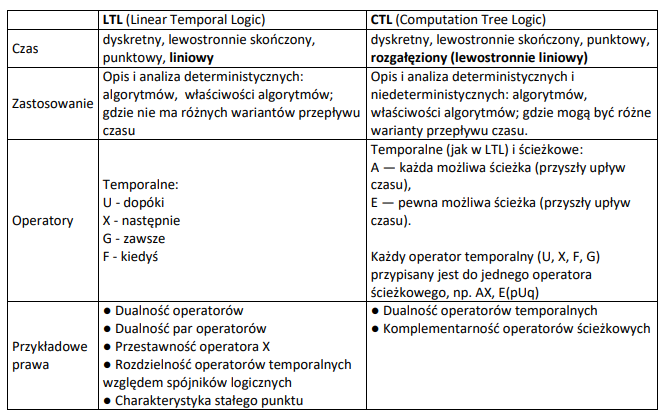
\includegraphics[width=0.8\linewidth]{K8.png}
	\caption{\textbf{LTL} vs \textbf{CTL}}
\end{figure}

\subsubsection{Zalety i wady}

\textbf{Zalety}:

\begin{itemize}
	\item pełna \textbf{automatyzacja} (po utworzeniu wymagań i zdefiniowaniu ograniczeń wystarczy uruchomić weryfikację),
	\item \textbf{łatwe dowodzenie} nieprawidłowości przez znalezienie kontrprzykładu. //
\end{itemize}

\textbf{Wady}

\begin{itemize}
	\item \textbf{złożoność obliczeniowa};eksplozja stanów,
	\item wykonanie abstrakcji \textbf{wymaga pracy eksperta}.
\end{itemize}

\subsubsection{Program współbieżny}

Współbieżny program składa się z procesów, gdzie:
\begin{itemize}
	\item procesy wykonywane są \textbf{w tym samym czasie},
	\item procesy mogą \textbf{współdzielić pewne zasoby}, np. zmienne,
	\item procesy mogą \textbf{wzajemnie oddziaływać} na siebie. \\
\end{itemize}

Własności programu:
\begin{itemize}
	\item \textbf{bezpieczeństwo} — q1 jest spełnione w \textbf{każdym} momencie,
	\item \textbf{osiągalność} — q2 będzie spełnione w \textbf{pewnym} momencie,
	\item \textbf{odpowiedź} — q3 jest spełnione od czasu do czasu,
	\item \textbf{trwałość} — od \textbf{pewnego momentu}: q4 jest spełnione \textbf{w każdym} momencie,
	\item \textbf{żywotność} — q5 jest osiągalne jako skutek p.
\end{itemize}

\subsubsection{Automat skończenie stanowy}

\begin{figure}[H]
	\centering
	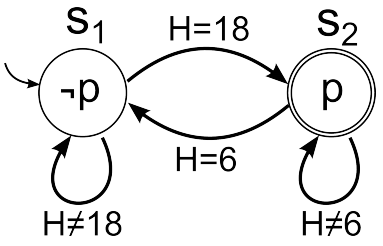
\includegraphics[width=0.4\linewidth]{K8_1.png}
	\caption{Automat skończenie stanowy - włączanie światła o 18.00 i wyłączanie 0 6.00}
\end{figure}

\begin{itemize}
	\item jest abstrakcyjną maszyną stanową,
	\item składa się ze skończonej liczby stanów i przejść między nimi,
	\item ma stany początkowe i może mieć stany końcowe,
	\item jest automatem, w którym przejścia między stanami są odpalane deterministycznie(jednoznacznie opisane funkcją przejścia).
\end{itemize}

\subsubsection{Modelowa weryfikacja systemu}

Dane wejściowe:
\begin{itemize}
	\item formalny \textbf{model funkcji systemu} dany \textbf{jako automat},
	\item \textbf{własności}, które muszą być spełnione przez system, dane \textbf{jako formuły logiki temporalnej}. \\
\end{itemize}

Dane wyjściowe:
\begin{itemize}
	\item \textbf{odpowiedź}, czy system spełnia te własności. \\
\end{itemize}

Najważniejsze własności do weryfikacji:
\begin{itemize}
	\item \textbf{osiągalność} — „pożądany” stan p systemu w końcu zostanie osiągnięty,
	\begin{itemize}
		\item LTL: $Fp$
		\item CTL: $EFp$
	\end{itemize}
	\item \textbf{bezpieczeństwo} — „niechciany” stan q systemu nigdy nie zostanie osiągnięty. 
	\begin{itemize}
		\item LTL: $G \lnot g$
		\item CTL: $AG \lnot g$
	\end{itemize}
\end{itemize}

\underline{\textbf{UPPAAL}}

\underline{\textbf{NuSMV}}
